\section{Week 1 - Introduction and NLP}
\subsection{Introduction}
\subsubsection{What is AI?}
A broad concept with different interpretations.
In this class: Where a computer \textbf{learns from data}.
Often called \textbf{statistical machine learning.}\\
Ultimate research goal: AGI (artificial general intelligence).
a hypothetical computer program that can perform intellectual tasks as well as, or better than, a human.

\subsubsection{AGI - Artificial General Intelligence}
Hypothetical computer program that can perform intellectual tasks as well as, or better, than a human.
\subsubsection{How to tell if a machine is intelligent}
With the \textbf{Turing Test:}\\
If the behaviour is indistinguishable from a human, it is intelligent.
Problems: AI must learn to lie, If a complex problem is too hard for humans.

\subsubsection{Applications of AI}
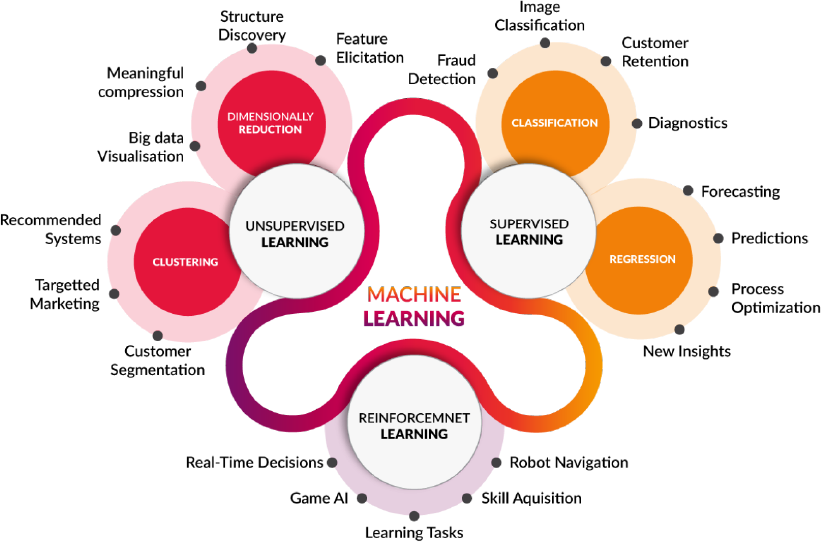
\includegraphics[width=\linewidth]{machine_learning_sections.png}
\includegraphics[width=\linewidth]{ai-einsatz.jpg}
\includegraphics[width=\linewidth]{ai-areas.jpg}
\begin{itemize}
    \item Personalization of news feeds
    \item Product searching and recommendation s on eCommerce platforms
    \item Voice-to-text
    \item Predictive maintenance
\end{itemize}

\subsection{NLP (Natural Language Processing)}
NLP is the \textbf{automated processing} of human language.
A Sub-field of AI, aiming to understand and generate language.
Long research history, took-off recently.
Still difficult, but Big-Business.
\subsection{Dialogflow}
\subsubsection{Intents}
What does the user want?
Give example sentences and Dialogflow will generate new sentences to match intent.

\subsubsection{Entities}
Extract information from sentence.
Assign words to entities (variables).
Again, define examples and dialogflow learns new words.

\subsubsection{Dialog Control}
\textbf{Linear:} Collect all Information, for e.g. booking an appointment
\textbf{Non-Linear:} More a real conversation with dependend answers based on changes in context.
Context can be set as Input and Ouput.
\subsubsection{Dialogflow Advanced}
\textbf{Intents}
\begin{itemize}
    \item Recognizes the need of a user
    \item Require training to match to user inputs
    \item Follow up Intents (on Success)
    \item Fallback Intents (on Failure)
\end{itemize}
\textbf{Entities}
\begin{itemize}
    \item Extract information from user inputs
    \item Help to identifiy required intent
    \item System Entities: (Date and time / Numbers / Amounts / Units / etc.)
    \item Developer Entities: defined by list of words (@pizza-type / @drink / etc.)
    \item User Entities: transient, temporary Information based on Conversation
\end{itemize}
\textbf{Dialog}
\begin{itemize}
    \item Linear: Gather a list of information
    \item Non Linear: Using Contexts
\end{itemize}
\textbf{Context}
\begin{itemize}
    \item Each Intent can have Input \& Output Context
    \item Intents are active based on active Context
    \item Expire automatically
\end{itemize}
\textbf{Fulfillment}
\begin{itemize}
    \item Action triggered on fullfilled Intents
    \item e.g. Webhook
\end{itemize}

\subsection{7 Steps of ML}
\begin{enumerate}
    \item Gathering data
    \item Preparing that data
    \item Choosing a model
    \item Training
    \item Evaluation
    \item Hyperparameter tuning
    \item Prediction
\end{enumerate}